
\section{Implementation}
\label{sec:Implementation}

\subsection{Komponenten}
\label{impl:Komponenten}

\subsection{QGIS Plugin}
\label{impl:QGIS Plugin}
TODO

\subsection{PlazaRoute Container}
\label{impl:PlazaRoute Container}
TODO

\subsubsection{Plaza Vorverarbeitung}
\label{impl:Plaza Vorverarbeitung}
TODO

\subsubsection{Plaza Routing}
\label{impl:Plaza Routing}
In den folgenden Unterkapitel wird die Umsetzung der Plaza Routing Architektur, welche im Kapitel \ref{architektur:Plaza Routing} definiert ist, erläutert. 

\paragraph{api}\label{impl:Plaza Routing api}~\\
In diesem Kapitel wird auf die Umsetzung der api-Schicht in Abbildung \ref{fig:package_diagram_plaza_routing} Bezug genommen.

TODO Flask Setup beschreiben

\paragraph{Zusammenspiel und Verantwortlichkeit}\label{impl:Plaza Routing Zusammenspielund Verantwortlichkeit}~\\
In Abbildung \ref{fig:sequence_diagram_plaza_routing_overview} sind die Interaktionen zwischen den Komponenten in einem Sequenz-Diagramm aufgeschlüsselt. Dabei wurde zur Wahrung der Übersichtlichkeit das Holen aller möglichen Routen in ein Unter-Squenz-Diagram in Abbildung \ref{fig:sequence_diagram_plaza_routing_route_combs} ausgelagert. Dabei geht es primär nicht um die Logik, die dahinter liegt, sondern um die Verantwortlichkeiten der Services. Wann sie ins Spiel kommen und für was sie benötigt werden, ist so gut ersichtlich.

\begin{figure}[ht]
    \centering
    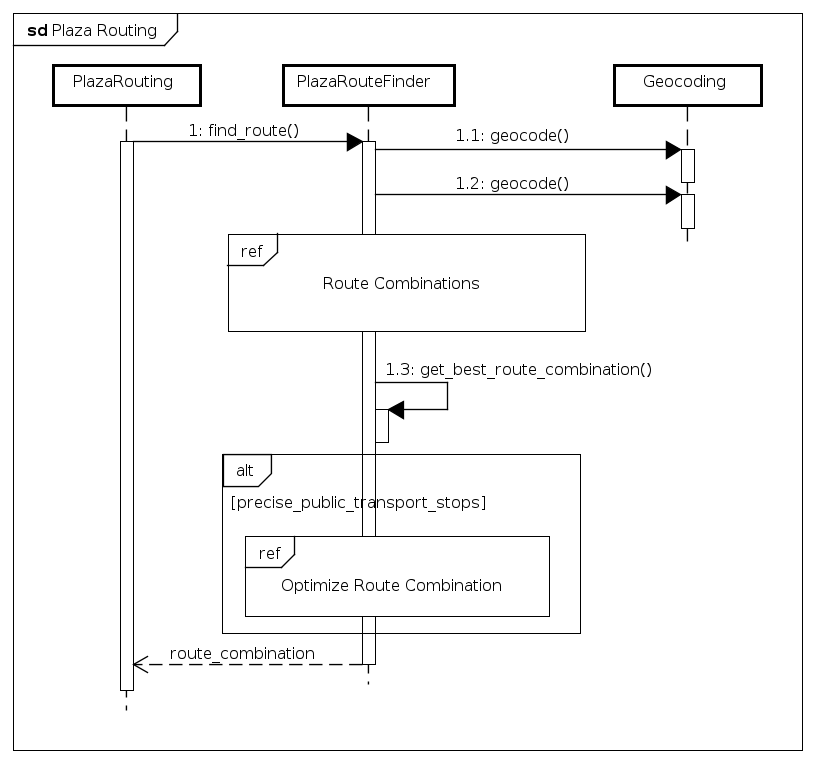
\includegraphics[width=0.7\linewidth]{projectdoc/img/sequence_diagram_plaza_routing_overview}
    \caption[Plaza Routing Sequenz-Diagramm Übersich]{Plaza Routing Sequenz-Diagramm Übersicht}
    \label{fig:sequence_diagram_plaza_routing_overview}
\end{figure}

\begin{figure}[ht]
    \centering
    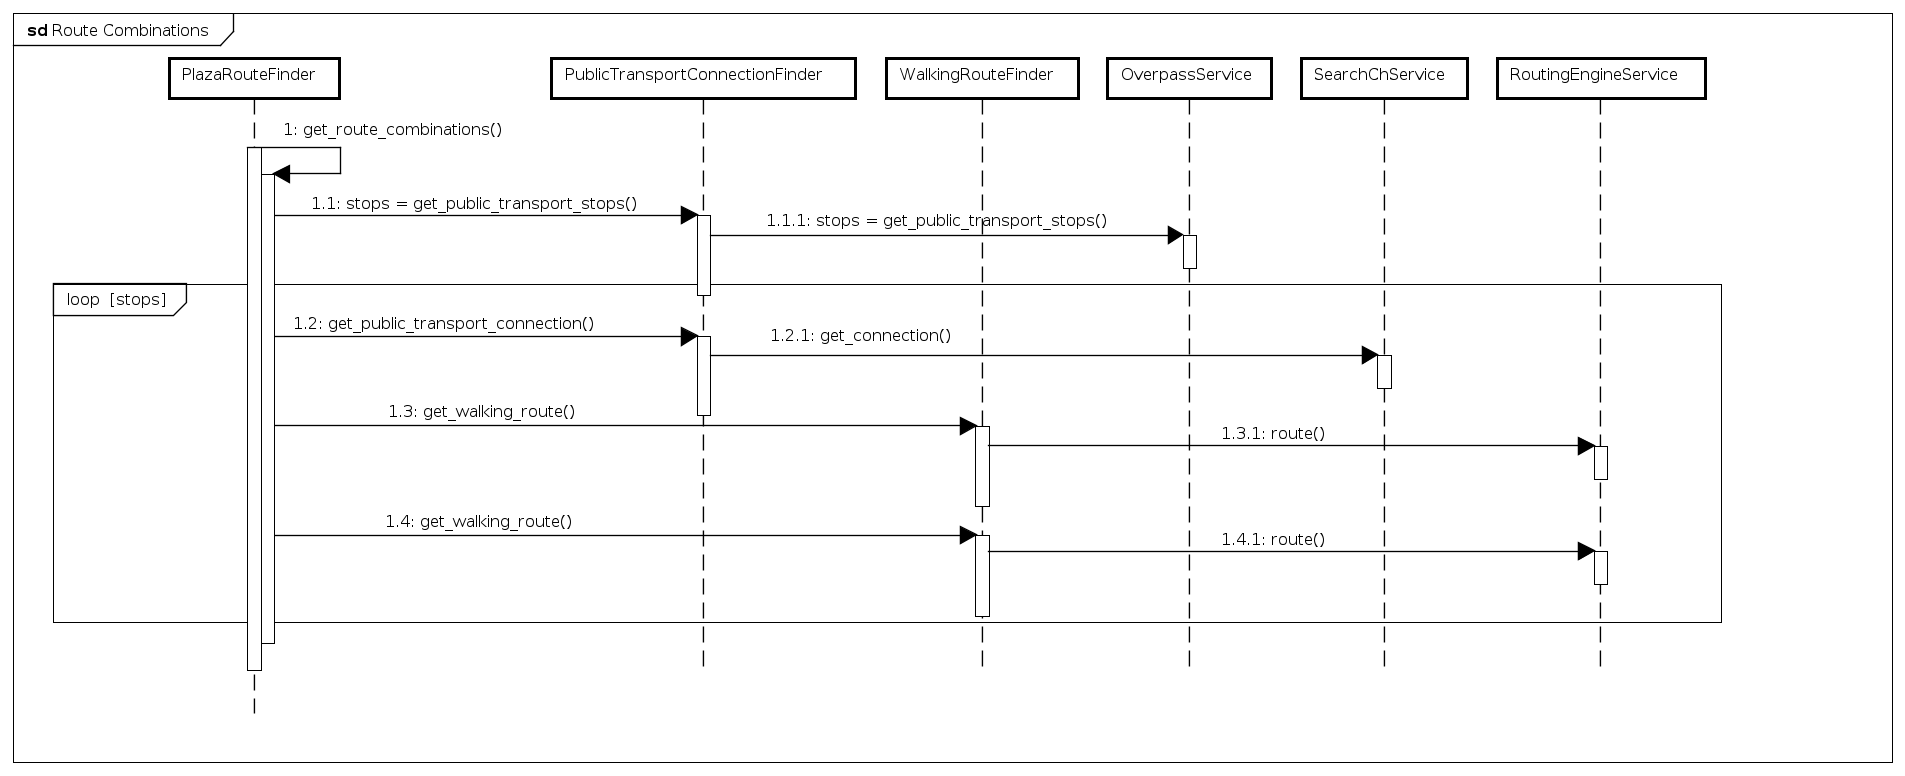
\includegraphics[width=1\linewidth]{projectdoc/img/sequence_diagram_plaza_routing_route_comb}
    \caption[Plaza Routing Sequenz-Diagramm Route Combinations]{Plaza Routing Sequenz-Diagramm Route Combinations}
    \label{fig:sequence_diagram_plaza_routing_route_combs}
\end{figure}

So sieht man in Abbildung \ref{fig:sequence_diagram_plaza_routing_route_combs} gut, dass im Loop für eine Ausgangs-ÖV-Station die Verbindung von search.ch \cite{search_ch_route_api} geholt (siehe \ref{impl:Plaza Routing ÖV-Haltestellen eruieren}) und zwei Mal eine Fussgänger-Routing durchgeführt wird, jeweils vom aktuellen Standort zur ersten ÖV-Station und von der letzten ÖV-Station zur Destination. Diese Daten sind die Grundlagen für die Entscheidungsfindung der besten Route, welches in \ref{impl:Plaza Routing Beste Route eruieren} beschrieben ist.

\paragraph{ÖV-Haltestellen eruieren}\label{impl:Plaza Routing ÖV-Haltestellen eruieren}~\\
ÖV-Haltestellen werden mit Overpass \cite{wiki:overpass} aus \ac{OSM} bezogen. Dabei wird um den aktuellen Standort eine \gls{BoundingBox} gezogen. Die Bounding Box ist konfigurierbar und entspricht einer zumutbaren Laufdistanz. In dieser Fläche werden Nodes und Relationen mit Tags, welche ÖV-Haltestellen identifizieren (\emph{''public\_transport''=''stop\_position''}, \emph{''type''=''public\_transport''} etc.), gefiltert und deren \emph{uic\_ref} zurückgegeben.

\paragraph{Beste Route eruieren}\label{impl:Plaza Routing Beste Route eruieren}~\\
% TODO was machen wir eigentlich, wenn zwei Verbindungen die gleichen Kosten haben?
Aufgrund der möglichen Routen, welche wie in Abbildung \ref{fig:sequence_diagram_plaza_routing_route_combs} gewonnen werden, muss man nun entscheiden, welche Route dem User konkret retourniert wird. Dazu wurde eine Kosten-Matrix erstellt. Diese ist in Tabelle \ref{table:cost-matrix} sichtbar.

\begin{table}[ht]
    \centering
    \begin{tabular}{l|l}
        & \textbf{Gewicht} \\ \hline
        \textbf{Gehzeit}                    & 2                \\
        \textbf{Dauer der ÖV-Verbindung}    & 1                \\
        \textbf{Anzahl der ÖV-Teilstrecken} & 7 * 60          
    \end{tabular}
    \caption{Kosten-Matrix}
    \label{table:cost-matrix}
\end{table}

Die Dauer des Fussstrecke wird doppelt gewichtet. Ein einmaliges Umsteigen schlägt mit 7 Minuten ins Gewicht. So lassen sich die Kosten aufgrund der Zeit, welche man für jeden Faktor benötigt, berechnen.

Eine Verbindung, bei welcher man 5 Minuten geht, 15 Minuten fährt und zwei Mal umsteigen muss, wird mit Totalkosten von \emph{5 * 60 * 2 + 15 * 60 + 2 * 7 * 60 = 2340} mit den anderen möglichen Verbindungen verglichen. Schlussendlich wird die Verbindung mit den niedrigsten Kosten retourniert.

\paragraph{Inkonsistentes ÖV-Mapping}\label{impl:Plaza Routing inkonsistentes ÖV-Mapping}~\\
Mit Hilfe von Overpass \cite{wiki:overpass} wird für eine ÖV-Verbindung die korrekte Koordinate der Einstiegs- und der letzten Endhaltestelle geholt. Search.ch \cite{search_ch_route_api} liefert in einer ÖV-Verbindung für zwei gegenüberliegenden Haltestelle (je eine für jede Fahrrichtung) eine Koordinate zurück, welche beispielsweise direkt auf der Hauptstrasse liegen kann (siehe Abbildung \ref{fig:one_coordinate_for_two_stops}). Dies ist für ein Fussgänger-Routing nicht optimal.

\begin{figure}[ht]
\centering
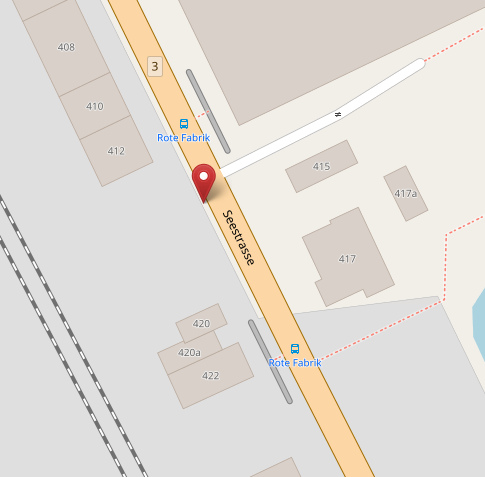
\includegraphics[width=0.5\linewidth]{projectdoc/img/one_coordinate_for_two_stops}
\caption[eine Koordinate für zwei ÖV-Stationen]{eine Koordinate für zwei ÖV-Stationen der Roten Fabrik, Zürich, Schweiz; openstreetmap.org; Screenshots aufgenommen am 25.11.2017}
\label{fig:one_coordinate_for_two_stops}
\end{figure}


Aus diesem Grund werden diese Koordinaten nun von Overpass \cite{wiki:overpass} bezogen. 
Da ÖV-Stationen und -Linien in \ac{OSM} jedoch nicht konsistent gemappt sind, wird das Recovery Blocks Pattern \cite{fault_tolerant_software} angewendet, um dem User so oft wie möglich ein genaues Resultat liefern zu können. Mit nicht konsistent meinen wir, dass sie nicht zwingend den Vorgaben in \cite{osm_wiki_relation} folgen. Durch Tests lassen sich jedoch Trends erkennen, wie Mapper grundsätzlich mit ÖV-Verbindungen umgehen.

Vorgängig muss klargestellt werden, dass wenn die Rede vo einer Linie ist, grundsätzliche eine Buslinie oder ähnliches, welches in \ac{OSM} als Relation \cite{osm_wiki_relation} abgebildet ist, gemeint ist. Spricht man von einer Station ist die ÖV-Station gemeint, welche als Node gemappt ist.

In einem ersten Schritt werden die Daten über die bekannte ÖV-Linie geladen. Search.ch \cite{search_ch_route_api} liefert eine uic\_ref für die initiale ÖV-Station und eine bei welcher man aussteigt. Üblicherweise erhält man zwei Relationen zurück, je eine für jede Fahrrichtung. Mit den beiden Stationen kann man nun die Members der Relation durchgehen und die Linie selektieren, bei welcher die uic\_ref der initialen ÖV-Station vor der uic\_ref der Ausstiegsstation kommt.
Anmerken muss man, dass es natürlich mit einem Risiko verbunden ist, so die korrekte Koordinate zu eruieren. Entspricht die Reihenfolge der Members nicht der Reihenfolge der ÖV-Stationen, ist aber obige Bedingungen trotzdem durch Zufall erfüllt, kann es vorkommen, dass man die falsche Station erwischt. Mit diesem Restrisiko leben wir.

Ist die erste Variante nicht erfolgreich, werden die Relationen mit der uic\_ref der initialen ÖV-Station geladen. ÖV-Stationen mit der gleichen uic\_ref gehören normalerweise zu einer Relation, welche auch diese uic\_ref besitzt. Über diese Relation können die möglichen initialen Ausgangsstationen und die Linien geladen werden. In einem weiteren Schritt werden die Ausstiegstationen in einem ähnlichen Verfahren für die uic\_ref der Ausstiegsstation geladen. Im idealen Fall hat man nun die Einstiegsstationen, Linien und Ausstiegstationen für beide Fahrtrichtungen. Mit diesen Daten kann nun die korrekte Einstiegs- und Ausstiegstation der konkreten Linie zugeordnet werden (durch ihre Zugehörigkeit als Member). Da man die Einstiegs- und Ausstiegstation separat geladen hat, ist es ein Leichtigkeit die Linie in die richtige Fahrtrichtung zu eruieren. 

Führen diese zwei Varianten nicht zum Ziel, wird die Koordinate von search.ch zurückgegeben.

Das Verbesserte Resultat von Abbildung \ref{fig:one_coordinate_for_two_stops} ist in Abbildung \ref{fig:one_coordinate_for_two_stops_improved} ersichtlich.

\begin{figure}[ht]
    \centering
    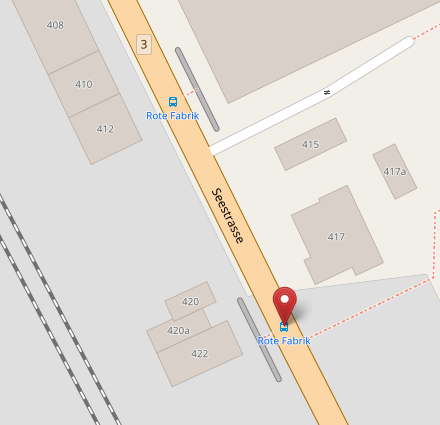
\includegraphics[width=0.5\linewidth]{projectdoc/img/one_coordinate_for_two_stops_improved}
    \caption[mit Overpass geladenen Koordinate]{mit Overpass geladenen Koordinate der Roten Fabrik in Richtung Seerose, Zürich, Schweiz; openstreetmap.org; Screenshots aufgenommen am 25.11.2017}
    \label{fig:one_coordinate_for_two_stops_improved}
\end{figure}


Die erhöhte Genauigkeit kommt nicht ohne Performanzeinbusse. Im Worst-Case wird drei Mal eine Overpass-Abfrage \cite{wiki:overpass} durchgeführt und schlussendlich doch die Fallback-Koordinate von search.ch \cite{search_ch_route_api} retourniert. Wir müssen uns nun die Frage stellen, welche Wartezeit dem User in diesem Fall noch zumutbar ist und ob der User entscheiden soll, ob er diese Genauigkeit will oder mit der Koordinate von search.ch \cite{search_ch_route_api} zufrieden ist.

